\documentclass[11pt,letterpaper]{article}
\usepackage[T1]{fontenc}
\usepackage[utf8]{inputenc}
\usepackage{amsthm}
\usepackage{newpxtext,newpxmath}
\usepackage[margin=1in,headheight=15pt]{geometry}
\usepackage{microtype,amsmath,amsthm,mathtools}
\usepackage{booktabs,array,longtable,graphicx}
\usepackage{xcolor,enumitem,fancyhdr,titlesec}
\usepackage[most]{tcolorbox}
\usepackage{listings,needspace}
\usepackage{hyperref}
\definecolor{Olive}{HTML}{526044}
\definecolor{Ink}{HTML}{26302A}
\definecolor{Sand}{HTML}{F5F4ED}
\definecolor{Rule}{HTML}{CDD1C3}
\hypersetup{colorlinks=true,linkcolor=Olive,citecolor=Olive,urlcolor=Olive,
 pdftitle={An explicit formula for lucky parking spots},
 pdfauthor={Research manuscript prepared for Vladimir Reshetnikov},
 pdfsubject={A proof of the polynomial-form conjecture for lucky parking spots}}
\titleformat{\section}{\Large\bfseries\color{Olive}}{\thesection}{0.7em}{}
\titleformat{\subsection}{\large\bfseries\color{Ink}}{\thesubsection}{0.6em}{}
\titlespacing*{\section}{0pt}{2.0ex plus 1ex}{1.1ex}
\titlespacing*{\subsection}{0pt}{1.6ex plus .6ex}{.7ex}
\pagestyle{fancy}
\fancyhf{}
\fancyhead[L]{\small\color{Olive}An explicit formula for lucky parking spots}
\fancyhead[R]{\small Research manuscript}
\fancyfoot[L]{\footnotesize 19 September 2026}
\fancyfoot[R]{\thepage}
\renewcommand{\headrulewidth}{0.3pt}
\setlength{\parskip}{0.35em}
\setlength{\parindent}{0pt}
\setlength{\emergencystretch}{2em}
\numberwithin{equation}{section}
\newtheorem{theorem}{Theorem}[section]
\newtheorem{lemma}[theorem]{Lemma}
\newtheorem{proposition}[theorem]{Proposition}
\newtheorem{corollary}[theorem]{Corollary}
\theoremstyle{definition}
\newtheorem{definition}[theorem]{Definition}
\newtheorem{remark}[theorem]{Remark}
\newcommand{\NN}{\mathbb N}
\newcommand{\QQ}{\mathbb Q}
\newcommand{\PP}{\mathbb P}
\newcommand{\EE}{\mathbb E}
\newcommand{\fall}[2]{(#1)_{\underline{#2}}}
\newcommand{\coef}[2]{[#1^{#2}]}
\DeclareMathOperator{\Bin}{Bin}
\DeclareMathOperator{\Pois}{Pois}
\DeclareMathOperator{\Res}{Res}
\newtcolorbox{resultbox}{colback=Sand,colframe=Rule,boxrule=.5pt,
 arc=1mm,left=10pt,right=10pt,top=7pt,bottom=7pt,breakable}
\lstset{basicstyle=\ttfamily\footnotesize,breaklines=true,columns=fullflexible,
 keepspaces=true,showstringspaces=false,frame=single,rulecolor=\color{Rule},
 backgroundcolor=\color{Sand},aboveskip=1em,belowskip=1em}

\begin{document}
\begin{titlepage}
\vspace*{0.5in}
{\small\sffamily\color{Olive}ENUMERATIVE COMBINATORICS \quad / \quad RESEARCH ARTICLE\par}
\vspace{0.3in}
{\Huge\bfseries\color{Ink}An explicit formula for\\[4pt]lucky parking spots\par}
\vspace{0.2in}
{\Large A proof of the polynomial-form conjecture,\\
with reflection identities and boundary asymptotics\par}
\vspace{0.25in}
{\large Prepared for Vladimir Reshetnikov\par}
{19 September 2026\par}
\vspace{0.35in}
\begin{abstract}
Let $C_{n,j}$ count ordinary parking functions on $n$ spots in which spot $j$
is occupied by a car that preferred that spot. We prove the explicit formula
\[
 C_{n,j}=\frac{j+1}{2j}(n+1)^{n-1}
 -\frac{1}{2j}\sum_{k=0}^{j-2}\binom nk j^k(n-j+1)^{n-1-k},
 \qquad 1\le j\le n,
\]
with the sum empty when $j=1$. Factoring the sum proves Conjecture 13 of
Butler, Hadaway, Lenius, Martens, and Moats, including the assertion that the
correction polynomial has degree exactly $j-2$. The leading coefficient is
$\frac1{2j}\sum_{k=0}^{j-2}j^k/k!$. The proof uses a last-arrival decomposition,
a bivariate exponential generating function, and two explicit applications
of Lagrange inversion.

The formula also gives an exact reflection law, formulas for every fixed
distance from the right endpoint, and in particular
\[
 C_{n,n-1}=\frac{(n+1)^{n-1}+(5n-1)(n-1)^{n-2}}4.
\]
A binomial-probability interpretation gives both edge limits in terms of
Poisson tails and proves convergence to $1/2$ whenever both distances to the
ends tend to infinity. Further consequences include a reciprocity identity
for the correction polynomials, a convergent fixed-column expansion in
$1/n$, and an exact central-column formula. All proofs are given in ordinary
mathematical language. The accompanying standard-library Python program
performs exact, independently organized checks and regenerates the data.
\end{abstract}
\vfill
{\small\color{Olive}Keywords: parking functions; lucky spots; tree function;
Lagrange inversion; binomial tails; OEIS A374756 and A374533.\par}
\end{titlepage}

\tableofcontents
\newpage

\section{The problem and the result}
\label{sec:main}

\subsection{What is being counted?}
Cars $1,\ldots,n$ arrive in this order at a one-way street with spots
$1,\ldots,n$. Car $i$ has a preference $a_i\in\{1,\ldots,n\}$ and parks at the
first unoccupied spot weakly to the right of $a_i$. A preference list is a
\emph{parking function} when all cars park successfully. A spot is
\emph{lucky} when the car occupying it preferred that very spot.

Write
\[
 P_n=(n+1)^{n-1}\quad(n\ge1),\qquad P_0=1,
\]
and let $C_{n,j}$ be the number of parking functions with lucky spot $j$.
Thus $p_{n,j}=C_{n,j}/P_n$ is a probability under the uniform distribution on
parking functions. The index $j$ denotes a \emph{spot}, not the arrival label
of a car. These two statistics are different.

Butler et al.\ \cite{butler} give formulas for the first five columns and
conjecture a polynomial form for every fixed column (Conjecture 13, p.~10).
Their Question 15 asks about columns at fixed distance from the right end.
The column triangle and the next-to-last column are associated with OEIS
A374756 and A374533, respectively \cite{oeis-triangle,oeis-next}.

\subsection{An explicit answer}
\begin{theorem}[Lucky-spot formula]\label{thm:main}
For every pair of integers $1\le j\le n$, put $x=n-j+1$. Then
\begin{equation}\label{eq:main}
 \boxed{\displaystyle
 C_{n,j}=\frac{j+1}{2j}P_n
 -\frac{1}{2j}\sum_{k=0}^{j-2}\binom nk j^k x^{n-1-k}.}
\end{equation}
The empty-sum convention makes this valid for $j=1$ as well.
For $j\ge2$, define the rational polynomial
\begin{equation}\label{eq:f}
 f_j(n)=\frac{1}{2j}\sum_{k=0}^{j-2}
           \binom nk j^k(n-j+1)^{j-2-k},
\end{equation}
where $\binom nk=\fall nk/k!$ is interpreted polynomially. Then
\begin{equation}\label{eq:conjecture}
 C_{n,j}=\frac{j+1}{2j}(n+1)^{n-1}
             -f_j(n)(n-j+1)^{n-j+1},
 \qquad n\ge j,
\end{equation}
and $f_j$ has degree exactly $j-2$, with leading coefficient
\begin{equation}\label{eq:r}
 r_j=\frac{1}{2j}\sum_{k=0}^{j-2}\frac{j^k}{k!}>0.
\end{equation}
\end{theorem}

The exact degree is important: merely bounding it above would not prove the
full conjecture. Here it follows immediately from \eqref{eq:f}, because
every summand has degree $j-2$ and positive leading coefficient. The remaining
work is to establish \eqref{eq:main} without assuming the conjectured form.
Sections~\ref{sec:decomposition}--\ref{sec:extraction} provide that proof.

For orientation, the first polynomials are
\begin{align*}
 f_2(n)&=\frac14,\\
 f_3(n)&=\frac{2n-1}{3},\\
 f_4(n)&=\frac{13n^2-26n+9}{8},\\
 f_5(n)&=\frac{(2n-3)(59n^2-177n+64)}{30},\\
 f_6(n)&=\frac{115n^4-920n^3+2436n^2-2384n+625}{12}.
\end{align*}
The cases through $j=5$ agree with the previously published formulas
\cite{butler}; the single expression \eqref{eq:f} produces every column.
For instance, it gives $C_{10,6}=1\,258\,181\,726$.

\subsection{Scope and provenance}
The consulted journal version is in volume 29 (2026), article 26.1.1; its
arXiv predecessor is 2412.07873, first submitted in December 2024. In those
versions the target is explicitly a conjecture. Targeted searches made on
19 September 2026 did not locate a published resolution. This is a statement
about the consulted sources, not a guarantee that no independent proof
exists elsewhere.

This manuscript supplies a complete proposed proof and exact checks, rather
than treating a finite data fit as a solution. The local-outcome counting
method is established machinery; related fixed-lucky-car enumeration is
discussed by Harris and Martinez \cite{harris}. No novelty is claimed for
Lagrange inversion, the tree function, or the basic outcome factorization.
The claimed contribution is the explicit lucky-\emph{spot} formula and the
consequences proved below. The proof has not been peer-reviewed or checked
in a proof assistant.

\section{A decomposition at the last arriving car}
\label{sec:decomposition}

\subsection{Preferences compatible with a fixed outcome}
An \emph{outcome permutation} is the permutation
$\sigma=(\sigma_1,\ldots,\sigma_n)$ in which car $\sigma_i$ occupies spot $i$.
For each $i$, define
\begin{equation}\label{eq:lengths}
 b_i=\max\bigl(\{k<i:\sigma_k>\sigma_i\}\cup\{0\}\bigr),
 \qquad \ell_i=i-b_i.
\end{equation}
Thus $b_i$ is the nearest spot to the left whose eventual occupant arrives
\emph{after} car $\sigma_i$.

\begin{lemma}[Outcome factorization]\label{lem:outcome}
For a fixed outcome $\sigma$, the possible preference of car $\sigma_i$ is
any integer in $\{b_i+1,\ldots,i\}$, independently for each $i$. Consequently
\begin{equation}\label{eq:weights}
 P_n=\sum_{\sigma\in\mathfrak S_n}\prod_{i=1}^n\ell_i,
 \qquad
 C_{n,j}=\sum_{\sigma\in\mathfrak S_n}\prod_{i\ne j}\ell_i.
\end{equation}
\end{lemma}
\begin{proof}
Immediately before car $\sigma_i$ arrives, every spot strictly between
$b_i$ and $i$ is occupied: its occupant has smaller arrival label. Spot $i$
is unoccupied, and if $b_i>0$ then spot $b_i$ is also unoccupied. A preference
at most $b_i$ cannot lead to spot $i$, because the car would encounter an
unoccupied spot no later than $b_i$. A preference greater than $i$ cannot
lead backwards to $i$. Every preference between $b_i+1$ and $i$ does lead to
$i$.

To justify independence, assign one permitted preference to each car and
run the cars in increasing arrival-label order. Inductively, all earlier
cars occupy their prescribed spots. The preceding argument then puts the
current car in its prescribed spot too. Hence the choices really are
independent and exhaust all preference lists for this outcome.

There are $\ell_i$ choices at spot $i$. Requiring spot $j$ to be lucky fixes
its car's preference to $j$, replacing that one factor by $1$ and leaving
all other factors unchanged.
\end{proof}

For example, $\sigma=(2,4,1,3)$ gives
$(\ell_1,\ell_2,\ell_3,\ell_4)=(1,2,1,2)$. There are four compatible parking
functions; two have lucky spot 2, and two have lucky spot 4. This small
example also illustrates why simply counting outcome permutations would
lose the required weights.

\subsection{Splitting the street}
Suppose the last arriving car, labeled $n$, occupies spot $a+1$. There are
$a$ spots to its left and $b=n-1-a$ to its right. Choose the left labels in
$\binom{n-1}{a}$ ways. After standardizing labels within each side, the left
and right outcomes are arbitrary outcomes of lengths $a$ and $b$.

The weight of the last car is $a+1$, because all preceding spots are already
occupied. For a car on the right, the last car supplies a permanent
not-yet-arrived boundary while that right-side car parks; subtracting $a+1$
from spot numbers gives exactly the ordinary right-subproblem lengths.
Thus there is no hidden interaction across the split.

Define a polynomial marking the \emph{location} of one lucky spot:
\begin{equation}\label{eq:Hn}
 H_n(z)=\sum_{j=1}^n C_{n,j}z^{j-1},\qquad H_0(z)=0.
\end{equation}
This is a sum of indicators over possible marked spots, not the generating
polynomial of the total number of lucky spots.

\begin{proposition}[Last-arrival recurrence]\label{prop:recurrence}
For $n\ge1$,
\begin{align}\label{eq:recurrence}
 H_n(z)=\sum_{a+b=n-1}\binom{n-1}{a}\bigl(
 &(a+1)H_a(z)P_b \notag\\[-3pt]
 &+(a+1)z^{a+1}P_aH_b(z)+z^aP_aP_b\bigr).
\end{align}
\end{proposition}
\begin{proof}
The marked spot is on the left, on the right, or is occupied by car $n$.
In the first two cases the last car has its unrestricted factor $a+1$.
A right-side marked spot is shifted by $a+1$ positions, giving $z^{a+1}$.
In the third case car $n$ itself is required to be lucky, so its factor is
$1$, and its spot contributes $z^a$. Lemma~\ref{lem:outcome} supplies the
remaining independent factors.
\end{proof}

The recurrence is already an exact algorithm for the entire triangle. It
will also provide a computational check that is independent of the final
binomial expression.

\section{The bivariate generating function}
\label{sec:gf}

\subsection{The tree function and Lagrange inversion}
Let $T=T(t)$ be the unique formal power series with zero constant term
satisfying
\begin{equation}\label{eq:tree}
 T=t e^T.
\end{equation}
The Lagrange inversion formula in the form needed here is
\begin{equation}\label{eq:lagrange}
 [t^m]F(T(t))=\frac1m[u^{m-1}]F'(u)e^{mu},\qquad m\ge1.
\end{equation}
For completeness, this follows by substituting $t=u e^{-u}$ in the formal
residue for the coefficient. The resulting residue is
$\Res F(u)(1-u)e^{mu}u^{-m-1}\,du$; the residue of the derivative of
$F(u)e^{mu}u^{-m}$ is zero, yielding \eqref{eq:lagrange}.

In particular,
\begin{equation}\label{eq:exp-tree}
 [t^m]e^{cT(t)}=\frac{c(m+c)^{m-1}}{m!}\quad(m\ge1),
 \qquad
 T(t)=\sum_{m\ge1}\tau_m t^m,
 \quad \tau_m=\frac{m^{m-1}}{m!}.
\end{equation}
This identity applies to positive or negative $c$; no analytic convergence
is needed for its formal use.

The familiar total $P_n=(n+1)^{n-1}$ can be counted by arranging $n+1$ spots
on a circle. All $(n+1)^n$ preference lists park, leaving one spot empty.
Rotating every preference rotates the empty spot, and every orbit has
exactly one list leaving spot $n+1$ empty. Such a list is precisely an
ordinary parking function on the first $n$ spots: no car can prefer or
traverse the spot that remains empty. Therefore
\begin{equation}\label{eq:P}
 P(t):=\sum_{n\ge0}P_n\frac{t^n}{n!}=e^{T(t)},
 \qquad T=tP(t),\qquad
 T'(t)=\frac{P(t)}{1-T(t)}.
\end{equation}
The coefficient identity also follows directly from \eqref{eq:exp-tree}
with $c=1$.

\subsection{A linear differential equation}
Set
\[
 H(z,t)=\sum_{n\ge0}H_n(z)\frac{t^n}{n!}.
\]
Multiplication of exponential generating functions absorbs the binomial
coefficient in \eqref{eq:recurrence}. Its three terms give
\[
 H_t=(H+tH_t)P(t)
   +z\bigl(P(zt)+ztP'(zt)\bigr)H+P(t)P(zt).
\]
Equivalently,
\begin{equation}\label{eq:ode-t}
 (1-T(t))H_t
 =\bigl(P(t)+\tfrac{d}{dt}T(zt)\bigr)H+P(t)P(zt).
\end{equation}
This is linear in $H$ and, with $H(z,0)=0$, determines it uniquely.

Make the change of variables
\[
 u=T(t),\qquad v=T(zt),\qquad t=u e^{-u}.
\]
Throughout a derivative in $u$ holds $z$ fixed. The identity
$v e^{-v}=z u e^{-u}$ gives
\begin{equation}\label{eq:vderivative}
 \frac{dv}{du}=\frac{v(1-u)}{u(1-v)},
 \qquad e^v=\frac{v e^u}{zu}.
\end{equation}
Equation~\eqref{eq:ode-t} becomes
\begin{equation}\label{eq:ode-u}
 H_u=\left(1+\frac{v}{u(1-v)}\right)H+e^v.
\end{equation}
A homogeneous solution is
\[
 L(u,z)=e^u\frac{u-v}{u},
 \qquad
 \frac{L_u}{L}=1+\frac{v}{u(1-v)}.
\]
Variation of constants therefore gives
\begin{equation}\label{eq:H-integral}
 H(z,t)=\frac{e^u(u-v)}{zu}
 \int_0^u\frac{T(zs e^{-s})}{s-T(zs e^{-s})}\,ds.
\end{equation}

All divisions in this expression have a harmless formal interpretation.
The series $T(zs e^{-s})/s$ is well-defined and divisible by $z$, so
$1-T(zs e^{-s})/s$ is invertible as a series in $z$. The integral is also
divisible by $z$, canceling the displayed $1/z$. Finally $(u-v)/u$ is
well-defined and has constant term $1-z$ in $u$. In particular, no assertion
about a singular analytic integral is being smuggled into the proof.

\section{Extracting the exact formula}
\label{sec:extraction}

\subsection{The first coefficient extraction}
For $j\ge1$, define
\begin{align}
 Q_j(s)&=\sum_{h=0}^{j-1}\left(1-\frac hj\right)\frac{(js)^h}{h!},
 \label{eq:Q}\\
 R_j(u)&=\sum_{h=0}^{j-1}
 \frac{(j-h)(j-h+1)}{2j^2}\frac{(ju)^h}{h!},
 \qquad c_j=\frac{j+1}{2j}.
 \label{eq:R}
\end{align}
Lagrange inversion in the variable $z$ gives
\begin{align}\label{eq:integrand-coefficient}
 [z^j]\frac{T(zs e^{-s})}{s-T(zs e^{-s})}
 &=\frac{(s e^{-s})^j}{j}
       [w^{j-1}]\frac{s e^{jw}}{(s-w)^2} \notag\\
 &=e^{-js}Q_j(s).
\end{align}
The last equality follows by expanding $(1-w/s)^{-2}$; the apparent negative
powers of $s$ cancel against $s^j$.

A direct differentiation of the polynomial \eqref{eq:R} shows that
$R_j'=jR_j-Q_j$ and $R_j(0)=c_j$. Hence, coefficientwise,
\begin{equation}\label{eq:I}
 I_j(u):=\int_0^u e^{-js}Q_j(s)\,ds=c_j-e^{-ju}R_j(u).
\end{equation}
Define
\begin{equation}\label{eq:S-convolution}
 S_j(u)=\sum_{a=1}^{j-1}\tau_a u^{a-1}R_{j-a}(u)-R_j(u).
\end{equation}
Since $v=\sum_{a\ge1}\tau_a z^a u^a e^{-au}$, extracting $z^{j-1}$
from \eqref{eq:H-integral} yields
\begin{equation}\label{eq:Hj}
 \begin{split}
 [z^{j-1}]H(z,t)
 =c_j e^u-\sum_{a=1}^{j-1}c_{j-a}\tau_a t^{a-1}
                 +e^{-(j-1)u}S_j(u).
 \end{split}
\end{equation}
The fact that $u^{a-1}e^{-(a-1)u}=t^{a-1}$ is essential here: the middle
expression is a finite polynomial in $t$, not an additional infinite
series contributing to large $n$.

\subsection{The convolution that makes the formula simple}
\begin{lemma}[Closed form of the auxiliary polynomial]\label{lem:S}
For $j\ge2$,
\begin{equation}\label{eq:S-closed}
 S_j(u)=\frac1{2j}\sum_{h=0}^{j-2}
      \frac{(ju)^h}{h!(j-h-1)}
      -\frac{j^{j-3}}{(j-1)!}u^{j-1}.
\end{equation}
Also $S_1(u)=-1$.
\end{lemma}
\begin{proof}
The degree of each summand in the convolution in \eqref{eq:S-convolution}
is at most $j-2$. Thus the coefficient of $u^{j-1}$ comes only from $-R_j$
and equals the last coefficient in \eqref{eq:S-closed}. The constant term,
for $j\ge2$, is
\[
 R_{j-1}(0)-R_j(0)
 =\frac{j}{2(j-1)}-\frac{j+1}{2j}
 =\frac1{2j(j-1)}.
\]
It remains to treat $1\le h\le j-2$.

Put $m=h+1$ and $c=j-m\ge1$. Expanding \eqref{eq:S-convolution}, the
convolution part of the coefficient of $u^h$ is
\begin{equation}\label{eq:convolution-coeff}
 \frac{c(c+1)}2
 \sum_{a=1}^{m}\frac{a^{a-1}}{a!}
               \frac{(j-a)^{m-a-2}}{(m-a)!}.
\end{equation}
Introduce the formal series
\[
 U_c(t)=\sum_{b\ge0}\frac{(b+c)^{b-2}}{b!}t^b.
\]
Multiplying the coefficient at $t^b$ by $b+c$ and using
\eqref{eq:exp-tree} shows that
\[
 tU_c'(t)+cU_c(t)=\frac1c e^{cT(t)}.
\]
Its constant term is $1/c^2$, and direct differentiation gives the unique
solution
\begin{equation}\label{eq:Uc}
 U_c(t)=e^{cT(t)}\left(\frac1{c^2}-\frac{T(t)}{c(c+1)}\right).
\end{equation}
The sum in \eqref{eq:convolution-coeff} is $[t^m]T(t)U_c(t)$.
Two applications of \eqref{eq:lagrange}, with $m+c=j$, give
\begin{align*}
 [t^m]T(t)e^{cT(t)}&=\frac{(c+1)j^{m-2}}{(m-1)!},\\
 [t^m]T(t)^2e^{cT(t)}&=\frac{(c+2)j^{m-3}}{(m-2)!}.
\end{align*}
The second identity is being used only for $m\ge2$.
Therefore the sum in \eqref{eq:convolution-coeff} equals
\[
 \frac{(c+1)j^{m-2}}{c^2(m-1)!}
 -\frac{(c+2)j^{m-3}}{c(c+1)(m-2)!}.
\]
After multiplication by $c(c+1)/2$ and subtraction of the coefficient of
$R_j$, the coefficient of $S_j$ is
\begin{align*}
 \frac{j^{m-3}}{2(m-1)!}
 \left(\frac{(c+1)^2j}{c}-(c+2)(m-1)-(c+1)(c+2)\right)
 &=\frac{j^{m-2}}{2c(m-1)!}\\
 &=\frac{j^{h-1}}{2h!(j-h-1)}.
\end{align*}
In the simplification we used $j=m+c$. This is exactly the coefficient
specified by \eqref{eq:S-closed}. Finally $S_1=-R_1=-1$ follows directly.
\end{proof}

\subsection{The final extraction and proof of the conjecture}
\begin{proof}[Proof of Theorem~\ref{thm:main}]
For $j=1$, equation~\eqref{eq:Hj} reads
$[z^0]H=e^{T(t)}-1$, so $C_{n,1}=P_n$ for $n\ge1$.
Suppose $j\ge2$. In \eqref{eq:Hj}, the middle polynomial has degree at most
$j-2$. The final term of \eqref{eq:S-closed}, after multiplication by
$e^{-(j-1)u}$, is a constant multiple of
$u^{j-1}e^{-(j-1)u}=t^{j-1}$. Neither contributes to $[t^n]$ for $n\ge j$.

The remaining terms, besides $c_je^{T(t)}$, are
\[
 \frac1{2j}\sum_{h=0}^{j-2}
 \frac{j^h}{h!(j-h-1)}t^h e^{-(j-h-1)T(t)}.
\]
Let $b=j-h-1>0$ and $m=n-h\ge1$. By \eqref{eq:exp-tree},
\[
 [t^m]e^{-bT(t)}=-\frac{b(m-b)^{m-1}}{m!}.
\]
Here $m-b=n-j+1=x\ge1$. Multiplying by $n!$ shows that the contribution
of the term indexed by $h$ is
\[
 -\frac1{2j}\binom nh j^h x^{n-1-h}.
\]
Adding these contributions proves \eqref{eq:main}.
Factoring $x^{n-j+1}$ gives \eqref{eq:f} and \eqref{eq:conjecture}.
Each term in \eqref{eq:f} has degree $j-2$ and leading coefficient
$j^k/(2j\,k!)$. Their sum is the strictly positive number \eqref{eq:r},
proving the exact degree and completing the proof.
\end{proof}

\begin{remark}[Why finite interpolation would have been insufficient]
Computing many values of $C_{n,j}$ and fitting a polynomial after dividing
by $x^{n-j+1}$ would only test the conjecture. The proof instead explains
why the infinite generating function collapses to the particular finite
binomial sum: the unwanted terms become polynomials in $t$ supported
strictly below $n=j$. This cancellation is the structural step, and
Lemma~\ref{lem:S} makes it explicit.
\end{remark}

\section{Binomial probabilities, reflection, and the right endpoint}
\label{sec:reflection}

\subsection{An exact probability representation}
\begin{corollary}[Binomial-tail representation]\label{cor:binomial}
Let $x=n-j+1$ and $Y\sim\Bin(n,j/(n+1))$. Then
\begin{equation}\label{eq:binomial}
 p_{n,j}=\frac{j+1}{2j}
       -\frac{n+1}{2jx}\PP(Y\le j-2).
\end{equation}
Equivalently,
\begin{equation}\label{eq:split-probability}
 p_{n,j}=\frac12+\frac1{2j}\PP(Y\ge j-1)
                    -\frac1{2x}\PP(Y\le j-2).
\end{equation}
\end{corollary}
\begin{proof}
Since $j+x=n+1$,
\[
 \PP(Y\le j-2)=\frac1{(n+1)^n}
             \sum_{k=0}^{j-2}\binom nk j^k x^{n-k}.
\]
Divide \eqref{eq:main} by $P_n$ and use
$(n+1)/(jx)=1/j+1/x$. The same calculation works for $j=1$ with
$\PP(Y\le-1)=0$.
\end{proof}

This binomial random variable is a representation of the final answer;
the proof does not assume that preference choices remain independent after
conditioning on successful parking.

\begin{theorem}[Reflection identity]\label{thm:reflection}
For $1\le j\le n$ and $x=n-j+1$,
\begin{equation}\label{eq:reflection}
 \boxed{\displaystyle
 C_{n,j}+C_{n,x}
   =P_n+\frac{n!}{j!\,x!}j^{j-1}x^{x-1}.}
\end{equation}
\end{theorem}
\begin{proof}
For $Y\sim\Bin(n,j/(n+1))$, the corresponding binomial variable for
column $x$ has the distribution of $n-Y$. Thus the two tail probabilities
appearing in \eqref{eq:binomial} are
$\PP(Y\le j-2)$ and $\PP(Y\ge j+1)$. Their sum is
$1-\PP(Y=j-1)-\PP(Y=j)$.

The two missing masses are equal, because
\[
 \frac{\PP(Y=j)}{\PP(Y=j-1)}
   =\frac{n-j+1}{j}\frac{j}{x}=1.
\]
The constant parts in the two formulas sum to
$1+(n+1)/(2jx)$. The tail coefficients are both $(n+1)/(2jx)$.
Consequently
\[
 p_{n,j}+p_{n,x}-1
  =\frac{n+1}{jx}\binom nj\frac{j^j x^{n-j}}{(n+1)^n}.
\]
Multiplication by $P_n$ and the identity $x!=(n-j+1)(n-j)!$ give
\eqref{eq:reflection}.
\end{proof}

The extra term has a direct relation to the last car. The number of parking
functions in which car $n$ is lucky at spot $j$ is
\[
 L_{n,j}=\binom{n-1}{j-1}P_{j-1}P_{n-j};
\]
this follows by splitting the street into the two completely filled sides
and fixing its final preference to $j$. Thus \eqref{eq:reflection} is also
$C_{n,j}+C_{n,n-j+1}=P_n+nL_{n,j}$.

\subsection{All fixed right-edge columns}
\begin{corollary}[Right-edge polynomial form]\label{cor:right}
For $j\ge2$, set
\begin{equation}\label{eq:g}
 g_j(n)=(n-j+1)f_j(n)+\frac{j^{j-1}}{j!}\fall n{j-1}.
\end{equation}
For every $n\ge j$,
\begin{equation}\label{eq:right}
 C_{n,n-j+1}=\frac{j-1}{2j}P_n
                 +g_j(n)(n-j+1)^{n-j}.
\end{equation}
The polynomial $g_j$ has degree $j-1$, with leading coefficient
\begin{equation}\label{eq:right-leading}
 r_j+\tau_j=\frac1{2j}\sum_{k=0}^{j}\frac{j^k}{k!}.
\end{equation}
For $j=1$, take $f_1=0$ and $g_1=1$, obtaining $C_{n,n}=n^{n-1}$.
\end{corollary}
\begin{proof}
Subtract \eqref{eq:conjecture} from \eqref{eq:reflection} and factor
$x^{n-j}$. This gives \eqref{eq:g}--\eqref{eq:right}. Both leading
coefficients in \eqref{eq:g} are positive. Finally the terms with indices
$j-1$ and $j$ in the sum in \eqref{eq:right-leading} are equal and each
is $j\tau_j$ before division by $2j$.
\end{proof}

In particular,
\begin{align}
 C_{n,n-1}
 &=\frac{(n+1)^{n-1}+(5n-1)(n-1)^{n-2}}4,
 && n\ge2,\label{eq:next-last}\\
 C_{n,n-2}
 &=\frac13(n+1)^{n-1}
   +\frac{13n^2-19n+4}{6}(n-2)^{n-3},
 && n\ge3.\label{eq:third-last}
\end{align}
Equation~\eqref{eq:next-last} gives a closed form for A374533, whose nine
listed values at the time of consultation are reproduced by the formula
\cite{oeis-next}. More generally, \eqref{eq:g} answers the fixed-distance
version of Question 15 by finite polynomial arithmetic, not by a recurrence
whose order grows with $n$.

\subsection{The central column and a row-sum check}
\begin{corollary}[Exact central probability]\label{cor:center}
For $m\ge1$,
\begin{equation}\label{eq:center}
 \frac{C_{2m-1,m}}{(2m)^{2m-2}}
      =\frac12+\frac1{m4^m}\binom{2m}{m}.
\end{equation}
\end{corollary}
\begin{proof}
Set $n=2m-1$ and $j=x=m$ in \eqref{eq:reflection}, then divide by twice
$P_n$. The remaining factorials simplify to the central binomial
coefficient in \eqref{eq:center}.
\end{proof}

Summing \eqref{eq:reflection} over $j$ also gives a useful global check.
From the last-car decomposition and \eqref{eq:P},
\[
 \sum_{j=1}^n L_{n,j}
  =(n-1)![t^{n-1}]P(t)^2=2(n+1)^{n-2}.
\]
The coefficient statement at $n=1$ is read directly as $1$; the displayed
closed expression also equals $1$ there. Hence
\begin{equation}\label{eq:row-sum}
 \sum_{j=1}^n C_{n,j}
    =P_n\frac{n(n+3)}{2(n+1)}.
\end{equation}
This counts marked lucky spots, not parking functions themselves, and is
consistent with the known expected lucky-car count because each lucky car
occupies exactly one lucky spot.

\section{Structure of the correction polynomials}
\label{sec:polynomials}

The expression \eqref{eq:f} is positive for integers $n\ge j$, even though
its expansion in ordinary powers of $n$ has alternating signs in the first
examples. In particular,
\[
 0<C_{n,j}<\frac{j+1}{2j}P_n\qquad(2\le j\le n).
\]
Positivity of $C_{n,j}$ also follows directly by taking any outcome with
all preferences equal to their final spots.

There is a second, less obvious structure. Put $m=j-2$. The polynomial
formula is equivalent to
\begin{equation}\label{eq:coefficient-polynomial}
 f_j(n)=\frac1{2j}[z^m]\frac{(1+jz)^n}{1-(n-j+1)z}.
\end{equation}
Here $(1+jz)^n$ is expanded by generalized binomial coefficients, so the
identity makes sense with $n$ an indeterminate.

\begin{proposition}[Polynomial reciprocity]\label{prop:reciprocity}
For $j\ge2$,
\begin{equation}\label{eq:reciprocity}
 f_j(j-2-n)=(-1)^{j-2}f_j(n).
\end{equation}
Thus $f_j(y+(j-2)/2)$ contains only powers of $y$ with the same parity as
$j-2$. For odd $j$, $2n-j+2$ is a factor of $f_j(n)$.
\end{proposition}
\begin{proof}
Write \eqref{eq:coefficient-polynomial} as a formal residue and substitute
$z=-w/(1+jw)$. This substitution has nonzero linear coefficient. Since
$m=j-2$ and $x=n-j+1$, it gives
\begin{align*}
 2j f_j(n)
 &=\Res_{z=0}\frac{(1+jz)^n}{1-xz}\frac{dz}{z^{m+1}}\\
 &=(-1)^m\Res_{w=0}
        \frac{(1+jw)^{m-n}}{1+(n+1)w}\frac{dw}{w^{m+1}}\\
 &=(-1)^m\,2j f_j(m-n).
\end{align*}
The final denominator is exactly the one associated with $n'=m-n$, since
$n'-j+1=-n-1$. Centering the variable gives the parity statement, and an
odd polynomial has a zero at its center.
\end{proof}

For example,
\begin{align*}
 f_4(y+1)&=\frac{13y^2-4}{8},\\
 f_5(y+3/2)&=\frac{y(236y^2-275)}{60},\\
 f_6(y+2)&=\frac{115y^4-324y^2+81}{12}.
\end{align*}
This explains the linear factors in the odd-column examples rather than
merely recording them.

For $j\ge3$, the coefficient of $n^{j-3}$ follows from the center of
symmetry:
\begin{equation}\label{eq:second-leading}
 f_j(n)=r_j n^{j-2}
       -\frac{(j-2)^2}{2}r_j n^{j-3}+O(n^{j-4}).
\end{equation}
For $j=2$, use $f_2=r_2=1/4$ instead. No assertion about the other zeros,
such as their reality, is needed or made here.

\Needspace{7\baselineskip}
\section{Boundary limits, bulk behavior, and expansions}
\label{sec:asymptotics}

\subsection{Fixed distance from either edge}
\begin{theorem}[The two edge limits]\label{thm:limits}
For each fixed $j\ge1$, let $Z_j\sim\Pois(j)$. Then
\begin{align}
 \rho_j:=\lim_{n\to\infty}p_{n,j}
 &=\frac{j+1}{2j}-\frac{e^{-j}}{2j}
                      \sum_{k=0}^{j-2}\frac{j^k}{k!}
  =\frac12+\frac1{2j}\PP(Z_j\ge j-1),
 \label{eq:left-limit}\\
 \beta_{j-1}:=\lim_{n\to\infty}p_{n,n-j+1}
 &=\frac{j-1}{2j}+\frac{e^{-j}}{2j}
                      \sum_{k=0}^{j}\frac{j^k}{k!}
  =\frac12-\frac1{2j}\PP(Z_j\ge j+1).
 \label{eq:right-limit}
\end{align}
In particular, $\rho_j>1/2$ and $\beta_{j-1}<1/2$ for every finite $j$.
\end{theorem}
\begin{proof}
For fixed $j$, a binomial random variable with parameters
$n$ and $j/(n+1)$ converges to $\Pois(j)$. At each fixed nonnegative integer
$k$, this follows directly from
\[
 \binom nk\left(\frac{j}{n+1}\right)^k
 \left(1-\frac{j}{n+1}\right)^{n-k}
       \longrightarrow e^{-j}\frac{j^k}{k!}.
\]
Only finitely many such masses occur in \eqref{eq:binomial}, proving
\eqref{eq:left-limit}.

Alternatively using the reflection identity, its extra term divided by
$P_n$ tends to $\tau_j e^{-j}$. Hence the right limit equals
$1-\rho_j+\tau_j e^{-j}$. Equation~\eqref{eq:right-leading} gives the
stated finite sum. The probability forms and strict inequalities follow
because both Poisson tails have positive probability.
\end{proof}

\begin{table}[htbp]
\centering
\caption{Limiting probabilities at fixed distance from the two endpoints.
The right column uses spot $n-j+1$, not spot $j$. Values are computed from
the proved finite sums.}
\label{tab:limits}
\begin{tabular}{rccc}
\toprule
$j$ & $r_j$ & $\rho_j$ (left) & $\beta_{j-1}$ (right)\\
\midrule
1 & $0$ & $1.0000000000$ & $0.3678794412$\\
2 & $1/4$ & $0.7161661792$ & $0.4191691040$\\
3 & $2/3$ & $0.6334752878$ & $0.4412053148$\\
4 & $13/8$ & $0.5952370868$ & $0.4536046169$\\
5 & $59/15$ & $0.5734974085$ & $0.4615960655$\\
6 & $115/12$ & $0.5595786250$ & $0.4671918985$\\
8 & $42037/720$ & $0.5429141077$ & $0.4745342088$\\
10 & $461843/1260$ & $0.5333590161$ & $0.4791519875$\\
\bottomrule
\end{tabular}
\end{table}

In particular,
\[
 \beta_0=e^{-1},\qquad
 \beta_1=\frac14+\frac54e^{-2},\qquad
 \beta_2=\frac13+\frac{13}{6}e^{-3}.
\]
As $j\to\infty$, the standardized variable $(Z_j-j)/\sqrt j$ tends to a
standard normal variable. One direct verification expands its characteristic
function as
$\exp\{j(e^{it/\sqrt j}-1-it/\sqrt j)\}\to e^{-t^2/2}$.
The thresholds $j-1$ and $j+1$ are both within $O(1)$ of the mean, so
\begin{equation}\label{eq:edge-large-j}
 \rho_j=\frac12+\frac1{4j}+o(j^{-1}),\qquad
 \beta_{j-1}=\frac12-\frac1{4j}+o(j^{-1}).
\end{equation}
These are iterated edge limits: first $n\to\infty$ with $j$ fixed, then
$j\to\infty$. The next subsection treats moving columns directly.

\begin{figure}[htbp]
\centering
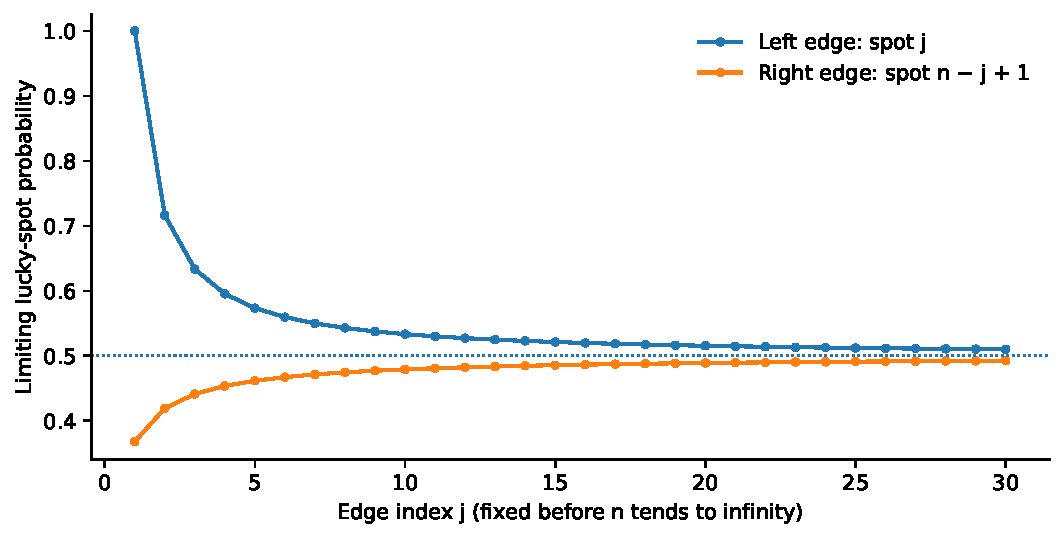
\includegraphics[width=.92\textwidth]{figures/boundary_limits.pdf}
\caption{The two fixed-edge limits from Theorem~\ref{thm:limits}. The plot
illustrates the proved formulas; it is not used to infer monotonicity.}
\end{figure}

\subsection{A uniform bulk limit}
\begin{corollary}[All columns escaping both endpoints]\label{cor:bulk}
For every $1\le j\le n$, with $x=n-j+1$,
\begin{equation}\label{eq:bounds}
 \frac12-\frac1{2x}\le p_{n,j}\le\frac12+\frac1{2j}.
\end{equation}
Consequently, for any sequence of column positions $j=j(n)$ such that
$j(n)\to\infty$ and $n-j(n)+1\to\infty$, one has
$p_{n,j(n)}\to1/2$.
\end{corollary}
\begin{proof}
Both tail probabilities in \eqref{eq:split-probability} lie in $[0,1]$.
The displayed bounds follow immediately and their errors tend to zero
under the stated hypotheses.
\end{proof}

No relation between the two rates of escape is required. For instance,
$j=\lfloor\log n\rfloor$ is covered, not just columns proportional to $n$.
If more specifically $j/n\to\alpha\in(0,1)$, the binomial central limit
theorem gives $\PP(Y\le j-2)\to1/2$: the threshold differs from the mean
by a bounded amount, whereas the standard deviation is of order $\sqrt n$.
Substitution in \eqref{eq:binomial} then yields the sharper limit
\begin{equation}\label{eq:bulk-first}
 n\left(p_{n,j}-\frac12\right)
 \longrightarrow\frac{1-2\alpha}{4\alpha(1-\alpha)}.
\end{equation}
For $\alpha=1/2$ this first correction vanishes, and the exactly centered
odd-size column has a different leading scale. From \eqref{eq:center} and
Stirling's expansion,
\begin{equation}\label{eq:center-asymptotic}
 p_{2m-1,m}=\frac12+\frac1{\sqrt\pi\,m^{3/2}}
 \left(1-\frac1{8m}+\frac1{128m^2}+O(m^{-3})\right).
\end{equation}
For clarity, this expansion follows by inserting
$\log(m!)=(m+\tfrac12)\log m-m+\tfrac12\log(2\pi)+1/(12m)
+O(m^{-3})$ into $(2m)!/(m!)^2$ and exponentiating. It is not obtained by
substituting a moving $j$ into a fixed-column expansion.

\begin{figure}[htbp]
\centering
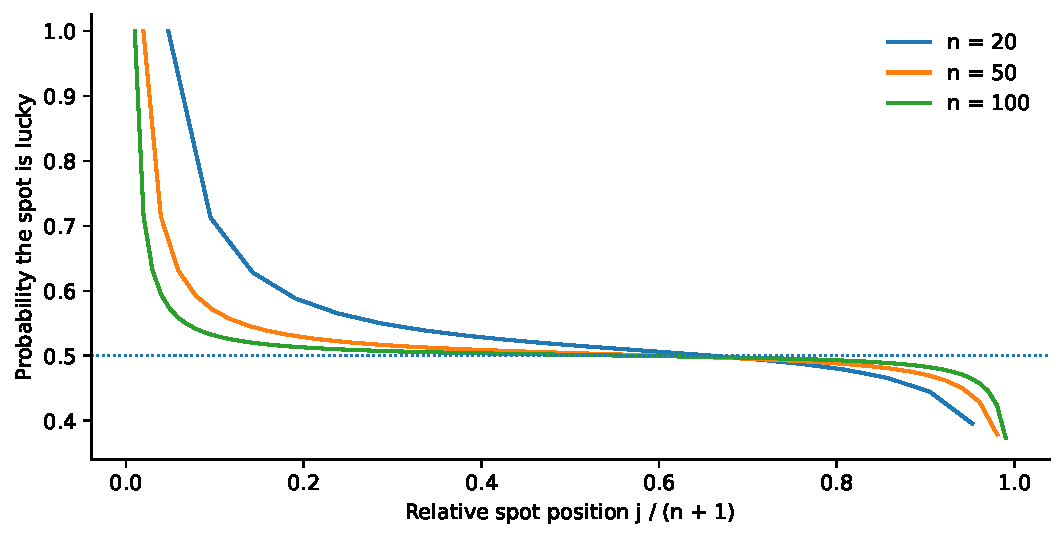
\includegraphics[width=.92\textwidth]{figures/probability_profiles.pdf}
\caption{Exact lucky-spot probabilities at three street lengths. The
near-end boundary regions coexist with convergence to $1/2$ in the interior.
All plotted counts were computed by exact integer arithmetic before
conversion to plotting coordinates.}
\end{figure}

\subsection{A convergent fixed-column expansion}
Fix $j\ge2$ and write $d=j-1$. An exact logarithmic expansion for $n>d$ is
\begin{equation}\label{eq:log-expansion}
 \begin{split}
 \log\left(
 n^{j-2}\frac{(n-d)^{n-d}}{(n+1)^{n-1}}
 \right)
 =-j+\sum_{q\ge1}
   \frac{d^{q+1}-(-1)^q(2q+1)}{q(q+1)n^q}.
 \end{split}
\end{equation}
To obtain it, expand $(n-d)\log(1-d/n)$ and
$(n-1)\log(1+1/n)$ and subtract. Both logarithmic series converge under the
stated inequality, so this is a convergent expansion, not just a formal
asymptotic rule.

Together with the finite polynomial $f_j(n)/n^{j-2}$, equation
\eqref{eq:log-expansion} provides every coefficient of the expansion of
$p_{n,j}$ in powers of $1/n$. Using \eqref{eq:second-leading}, the first
correction simplifies to
\begin{equation}\label{eq:first-correction}
 p_{n,j}=\rho_j-\frac{j r_j e^{-j}}{n}+O(n^{-2}).
\end{equation}
Indeed, the exponential contributes $(d^2+3)/(2n)$, and the polynomial
contributes $-(j-2)^2/(2n)$. Their sum is $j/n$. The same calculation with
the constant polynomial handles $j=2$.

The positive coefficient shows that, for each fixed $j\ge2$, the
probabilities approach their limiting value from below once $n$ is large
enough. This does not by itself prove monotonicity in $n$, and no such
stronger assertion is required here.

\section{Exact computations and reproducibility}
\label{sec:verification}

\subsection{Independent routes to the same counts}
The archive includes \texttt{code/verify.py}, which uses only the Python
standard library. Its count comparisons use integers and rational numbers;
no floating-point tolerances enter any pass/fail decision. It compares
four independently organized enumerations:

\begin{enumerate}[leftmargin=1.5em,itemsep=.3em]
\item Direct simulation of every preference list in $\{1,\ldots,n\}^n$.
A failed car rejects the list; successful cars directly record which spots
were lucky.
\item A dynamic program on the occupied-spot bitmask. For every state it
tries each possible next preference and accumulates both the number of
histories and the vector of lucky-spot counts.
\item Enumeration of outcome permutations with the factors
\eqref{eq:lengths}, checking Lemma~\ref{lem:outcome} against direct dynamics.
\item The last-arrival recurrence \eqref{eq:recurrence}, compared against the
closed expression \eqref{eq:main}.
\end{enumerate}
The first two methods use the parking process itself; they do not assume
the outcome-weight lemma or the final formula. The recurrence and the
closed form are distinct algorithms, although the proof explains their
connection.

\begin{table}[htbp]
\centering
\caption{Executed verification coverage. Every listed check passed.}
\label{tab:verification}
\begin{tabular}{p{.60\textwidth}p{.29\textwidth}}
\toprule
Check & Executed range\\
\midrule
Closed formula versus last-arrival recurrence & all $1\le j\le n\le100$;
$5\,050$ pairs\\
Reflection identity & the same $5\,050$ pairs\\
Exhaustive preference-list simulation & $n\le7$;
$873\,612$ lists\\
Direct occupied-state dynamic program & $n\le12$\\
Weighted outcome permutations & $n\le8$;
$46\,233$ permutations\\
Polynomial coefficients, exact degree, parity, and Lemma~\ref{lem:S}
& $2\le j\le30$\\
Published table prefixes and A374533 & 10 row prefixes; 9 terms\\
First/last columns, row sums, next-to-last formula, central formula
& all applicable $n\le100$\\
\bottomrule
\end{tabular}
\end{table}

A machine-readable transcript in \texttt{data/verification.json} records
these bounds and the actual interpreter version. The run used Python
3.13.5 and completed in approximately two seconds in the working
environment; timing is incidental, not a benchmark claim.

\Needspace{23\baselineskip}
\subsection{Minimal exact evaluator}
The final formula requires very little code. This evaluator uses only
integer arithmetic and explicitly checks divisibility:

\begin{minipage}{\linewidth}
\begin{lstlisting}[language=Python]
from math import comb

def lucky_spot_count(n: int, j: int) -> int:
    if not 1 <= j <= n:
        raise ValueError("Expected 1 <= j <= n")
    x = n - j + 1
    correction = sum(
        comb(n, k) * j**k * x**(n - 1 - k)
        for k in range(j - 1)
    )
    numerator = (j + 1) * (n + 1)**(n - 1) - correction
    value, remainder = divmod(numerator, 2 * j)
    if remainder:
        raise ArithmeticError("Unexpected nonintegral count")
    return value
\end{lstlisting}
\end{minipage}

For a single count this has $j-1$ summands, with additional cost for
large-integer arithmetic and exponentiation. Reflection permits evaluation
through the nearer endpoint. It is important not to describe such a bound
as constant-time arithmetic for arbitrarily large $n$: the output itself
has $\Theta(n\log n)$ bits.

For all rows through $N$, the straightforward last-arrival recurrence uses
$O(N^3)$ arithmetic operations and $O(N^2)$ stored integers. These are
arithmetic-operation bounds; bit complexity grows with the integer sizes.
The explicit formula is especially convenient for a fixed column or a fixed
distance from the right edge.

\subsection{Archive contents and commands}
The package contains the complete \LaTeX{} source and compiled PDF;
\texttt{verify.py}; optional plotting code; CSV data for all
$5\,050$ entries through $n=100$; exact rational polynomial coefficients
through $j=30$; 50-digit edge-limit tables; and a local extension of A374533.
The figure PDFs are vector graphics. No external fonts or copies of the
cited papers are redistributed.

From the package directory, run
\begin{lstlisting}
python code/verify.py
python code/make_figures.py      # optional; requires matplotlib
pdflatex -interaction=nonstopmode article.tex
pdflatex -interaction=nonstopmode article.tex
\end{lstlisting}
The first command needs Python 3.9 or later and no third-party packages.
The verification bounds can be changed with command-line options described
by \texttt{python code/verify.py --help}. A normal \TeX{} Live or MiK\TeX{}
installation with the packages named in the source can compile the article.
The supplied figures mean plotting is not necessary to rebuild the PDF.

\subsection{An OEIS indexing caution}
The consulted A374756 entry labels its statistic as a lucky \emph{car} in
the headline, while its comment and displayed triangle specify a lucky
\emph{spot}. Its longer example also reproduces only the first six columns
of the later rows. Our comparison therefore uses the stated $(n,j)$
coordinates and the published row prefixes, not an assumed flattening of
an incomplete triangle. The generated CSV supplies the complete triangular
array through $n=100$. A374533 has offset $n=2$ and is unambiguous
\cite{oeis-triangle,oeis-next}.

\section{Conclusion and remaining directions}
\label{sec:conclusion}
The selected target admits an explicit solution. The key result is not
merely the existence of a correction polynomial but the formula
\[
 f_j(n)=\frac1{2j}\sum_{k=0}^{j-2}\binom nk j^k(n-j+1)^{j-2-k}.
\]
It proves the exact degree, identifies the formerly unspecified rational
coefficient in the limiting probability, and reveals binomial tails behind
the column counts. The reflection identity then transfers fixed-column
information to the opposite endpoint, including the next-to-last-column
question, without a separate case analysis.

The resulting asymptotic picture is also precise. Fixed left-edge columns
have limiting probability greater than $1/2$; fixed right-edge columns have
limiting probability less than $1/2$; and every sequence of columns escaping
both ends converges to $1/2$. At the exact center, the first nonzero
correction has scale $n^{-3/2}$ rather than $n^{-1}$.

There are natural extensions, but they are not prerequisites for the
results proved here. A direct bijective explanation of the binomial tail
or the reflection identity would complement the generating-function proof.
Marking several specified lucky spots would lead to joint probabilities
and correlations; the present one-mark recurrence does not already solve
that problem. Finally, monotonicity questions and a uniform higher-order
transition expansion between edge and bulk regimes merit separate
arguments. Numerical patterns alone should not be promoted to theorems.

The mathematical conclusions of this manuscript rest on the displayed
proofs. The accompanying finite checks are intended to expose indexing,
weighting, and algebraic errors, and to make independent examination easy.
They are not substituted for those proofs.

\begin{thebibliography}{9}
\bibitem{butler}
S.~Butler, K.~Hadaway, V.~Lenius, P.~Martens, and M.~Moats,
\emph{Lucky Cars and Lucky Spots in Parking Functions},
Journal of Integer Sequences \textbf{29} (2026), Article 26.1.1.
Conjecture 13 and Question 15.
\url{https://cs.uwaterloo.ca/journals/JIS/VOL29/Hadaway/had3.pdf}.
Preprint: arXiv:2412.07873 (2024),
\url{https://arxiv.org/abs/2412.07873}.

\bibitem{oeis-triangle}
The OEIS Foundation Inc., \emph{The On-Line Encyclopedia of Integer Sequences},
A374756, lucky-spot triangle (see the entry's comment and example).
\url{https://oeis.org/A374756}. Accessed 19 September 2026.

\bibitem{oeis-next}
The OEIS Foundation Inc., \emph{The On-Line Encyclopedia of Integer Sequences},
A374533, parking functions whose next-to-last spot is lucky.
\url{https://oeis.org/A374533}. Accessed 19 September 2026.

\bibitem{harris}
P.~E.~Harris and L.~Martinez,
\emph{Parking functions with a fixed set of lucky cars},
arXiv:2410.08057v1 (2024), especially the outcome-counting formulation
in Theorem 2.6.
\url{https://arxiv.org/abs/2410.08057}.
\end{thebibliography}
\end{document}
